\begin{figure}[htbp]
\centering
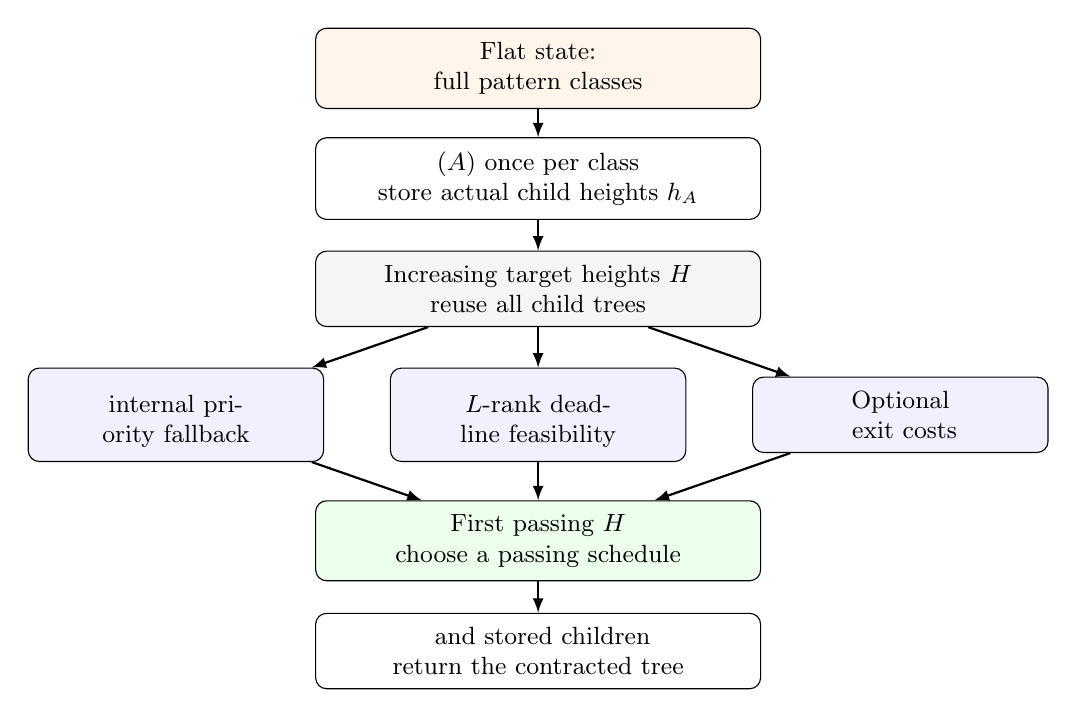
\begin{tikzpicture}[every node/.style={font=\small},
  box/.style={draw,rounded corners,align=center,inner sep=5pt,text width=3.4cm},
  wide/.style={box,text width=5.3cm},arr/.style={-latex,thick}]
  \node[wide,fill=orange!8] (hull) at (0,0)
    {Flat state: \HullData\\full pattern classes};
  \node[wide] (children) at (0,-1.4)
    {\HybridTree$(A)$ once per class\\store actual child heights $h_A$};
  \node[wide,fill=gray!8] (trial) at (0,-2.8)
    {Increasing target heights $H$\\reuse all child trees};
  \node[box,fill=blue!6] (priority) at (-4.6,-4.4)
    {\PriorityTrial\\internal priority fallback};
  \node[box,fill=blue!6] (slots) at (0,-4.4)
    {\SlotDP\\$L$-rank deadline feasibility};
  \node[box,fill=blue!6] (whole) at (4.6,-4.4)
    {Optional \SlotDP\\\EndpointCode\ exit costs};
  \node[wide,fill=green!7] (pass) at (0,-6)
    {First passing $H$\\choose a passing schedule};
  \node[wide] (attach) at (0,-7.4)
    {\EndpointCode\ and stored children\\return the contracted tree};
  \draw[arr] (hull) -- (children);
  \draw[arr] (children) -- (trial);
  \draw[arr] (trial) -- (priority);
  \draw[arr] (trial) -- (slots);
  \draw[arr] (trial) -- (whole);
  \draw[arr] (priority) -- (pass);
  \draw[arr] (slots) -- (pass);
  \draw[arr] (whole) -- (pass);
  \draw[arr] (pass) -- (attach);
\end{tikzpicture}
\caption{At a flat state, the algorithm first computes the hull and
children, then tests increasing target heights using three schedule
checks. The arrows carry the geometry, child heights, and candidate
schedules needed by those checks. The logarithmic cap $L$ is fixed at
the original root. The priority fallback guarantees a passing trial
by the stated height bound; the exact and whole-exit checks can certify
an earlier trial, and the algorithm selects the first trial accepted
by its explicit checks.}
\label{fig:hybrid-procedure-flow}
\end{figure}

